\documentclass{jlreq}

\usepackage{titlesec}
\usepackage{listings}
\usepackage{fancyhdr}

% url
\usepackage{url}

% \adjustbox
\usepackage{adjustbox}

% tcolorboxの設定
\usepackage[most]{tcolorbox} 
\tcbuselibrary{breakable}
\tcbuselibrary{skins}
\tcbuselibrary{listingsutf8}
% タイトルのフォーマットを変更
\titleformat{\title}
  {\centering\Huge\bfseries}
  {}
  {0em} 
  {}

\titleformat{\subtitle}
  {\centering\Large\itshape}
  {}
  {0em}
  {}

\titleformat{\subsubsection}[block]
  {\normalfont\normalsize\bfseries}
  {\arabic{subsubsection}.}
  {1em}
  {}

\titleformat{\section}[block]
  {\normalfont\large\bfseries}
  {\Roman{section}.}
  {1em} 
  {}
  [\titleline{\titlerule[1pt]}]

\titleformat{\subsection}[block]
  {\normalfont\normalsize\bfseries}
  {\roman{subsection}.}
  {1em}
  {}

% listingsの設定

\renewcommand{\lstlistingname}{コード}

\lstset{
	breaklines = true,
	language = Python,
	keywordstyle = {\bfseries \color[cmyk]{0,1,0,0}},
	commentstyle = {\itshape \color[cmyk]{1,0.4,1,0}},
	numbers = left,
	numberstyle = \tiny,
	stepnumber = 1,
	% frameとnumberの間の距離
	numbersep = 10pt,
	frame = single,
	basicstyle = \ttfamily,
	tabsize = 2,
	captionpos = t,
	backgroundcolor={\color[gray]{.90}},
	showstringspaces = false,
}

% headerの設定
\pagestyle{fancy}
\fancyhf{}

\fancyhead[RO,RE]{\rightmark}
\fancyhead[LO,LE]{\leftmark} 
\fancyfoot[C]{\thepage}

% tikzの設定
\usepackage{tikz}

\begin{document}
探索の章で扱うアルゴリズムは以下と通りです。

\begin{itemize}
  \item 線形探索
  \item 二分探索
  \item 二分探索木
  \item Treeq
  \item 平衡木(AVL木、B木、赤黒木)
  \item ハッシュ法
\end{itemize}

検索(サーチ)とは、データ集合(配列など)から、目的とする値を持った要素を探し出すことを意味する。

\section{線形探索}

\textbf{線形探索}は、目的とする要素が見つかるまで先頭から順に要素を見ていく探索方法です。例えば、以下の配列で0を探すなら前から順番に、
8, 4, 5, 0, 2の順に要素を見ていきます。

\vspace{0.5cm}

\begin{center}
  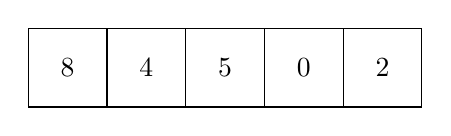
\begin{tikzpicture}
      \draw (0, 0) rectangle (1, 1);
      \node at (0.5, 0.5) {8};
      
      \draw (1, 0) rectangle (2, 1);
      \node at (1.5, 0.5) {4};
      
      \draw (2, 0) rectangle (3, 1);
      \node at (2.5, 0.5) {5};
      
      \draw (3, 0) rectangle (4, 1);
      \node at (3.5, 0.5) {0};
      
      \draw (4, 0) rectangle (5, 1);
      \node at (4.5, 0.5) {2};
  \end{tikzpicture}
\end{center}

\subsection{線形探索の実装}
\begin{lstlisting}[caption=線形探索の実装, frame=TRBL, label={linear}]
def linear_search(array: list[int], value: int) -> int:
    """
    線形探索をして一致するならそのindexを返す. 一致しないときは-1を返す
    """
    for i in range(len(array)):
        if array[i] == value:
            return i
    
    return -1


\end{lstlisting}

\subsection{番兵}

番兵法では探索するデータ集合の最後に目的とする数を追加します。最後に番兵を追加することで、より効率的に探索を行うことができます。
実際には番兵を追加してもそこまで効率が良くなるわけではないですが、番兵を追加することで、ループの条件判定を省略することができます。

\vspace{0.5cm}

\begin{center}
  \begin{tikzpicture}
      \draw (0, 0) rectangle (1, 1);
      \node at (0.5, 0.5) {8};
      
      \draw (1, 0) rectangle (2, 1);
      \node at (1.5, 0.5) {4};
      
      \draw (2, 0) rectangle (3, 1);
      \node at (2.5, 0.5) {5};
      
      \draw (3, 0) rectangle (4, 1);
      \node at (3.5, 0.5) {3};
      
      \draw (4, 0) rectangle (5, 1);
      \node at (4.5, 0.5) {2};
      
      \draw (5, 0) rectangle (6, 1);
      \fill[red, overlay] (5, 0) rectangle (6, 1);
      \node[white] at (5.5, 0.5) {0};
      \node[] at (5.5, -0.5) {番兵};
  \end{tikzpicture}
\end{center}

\begin{lstlisting}[caption=番兵の実装, frame=TRBL, label={sentinel}]
def linear_search(array: list[int], value: int) -> int:
    """
    線形探索をして一致するならそのindexを返す. 一致しないときは-1を返す
    """
    i = 0
    copied_array = array.copy()
    copied_array.append(value)
    while copied_array[i] != value: i += 1
    
    return i if i < len(array) else -1
  \end{lstlisting}

\section{二分探索}

\subsection{配列を探索する二分探索}

二分探索はソートされた配列に対して高速に探索を行うアルゴリズムの一つです。二分探索では探索する区間が条件に応じてどんどん半分になっていくため、
計算量は$O(\log n)$となります。以下の配列に対して、二分探索で18を探す場合を考えましょう。

最初の区間は配列全体を取ります。0-indexedな配列を考えると、midは39となり目的の18より大きいです。midが目的の値より大きい場合、
右の区間を狭めます。right = mid - 1とします。

\vspace{0.5cm}

\begin{center}
  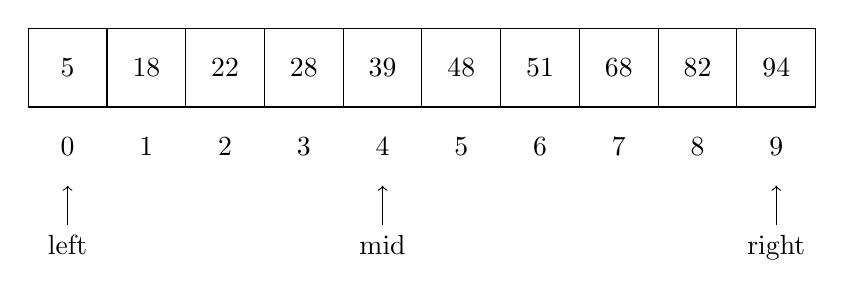
\begin{tikzpicture}
      \draw (0, 0) rectangle (1, 1);
      \node at (0.5, 0.5) {5};
      
      \draw (1, 0) rectangle (2, 1);
      \node at (1.5, 0.5) {18};
      
      \draw (2, 0) rectangle (3, 1);
      \node at (2.5, 0.5) {22};
      
      \draw (3, 0) rectangle (4, 1);
      \node at (3.5, 0.5) {28};
      
      \draw (4, 0) rectangle (5, 1);
      \node at (4.5, 0.5) {39};
      
      \draw (5, 0) rectangle (6, 1);
      \node at (5.5, 0.5) {48};
      
      \draw (6, 0) rectangle (7, 1);
      \node at (6.5, 0.5) {51};
      
      \draw (7, 0) rectangle (8, 1);
      \node at (7.5, 0.5) {68};
      
      \draw (8, 0) rectangle (9, 1);
      \node at (8.5, 0.5) {82};
      
      \draw (9, 0) rectangle (10, 1);
      \node at (9.5, 0.5) {94};

      \foreach \i in {0,1,...,9} {
        \node at (\i+0.5, -0.5) {\i};
    }

      % ラベルをはる
      \draw[<-] (0.5, -1) -- (0.5, -1.5) node[below] {left};
      \draw[<-] (9.5, -1) -- (9.5, -1.5) node[below] {right};
      \draw[<-] (4.5, -1) -- (4.5, -1.5) node[below] {mid};
  \end{tikzpicture}
\end{center}

\vspace{0.5cm}

rightを3に更新しました。mid = (0 + 3) // 2 = 1となります。midの値は18で目的の値と一致します。

\vspace{0.5cm}

\begin{center}
  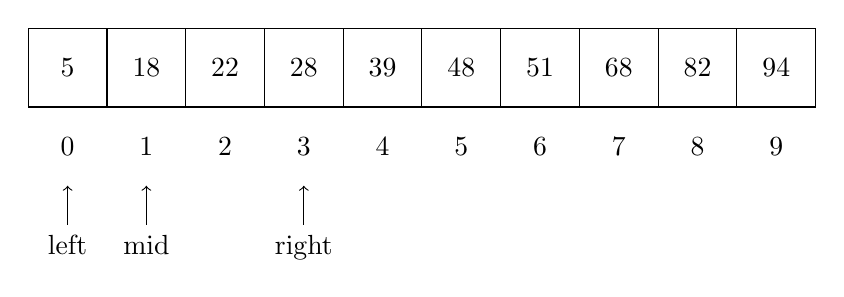
\begin{tikzpicture}
      \draw (0, 0) rectangle (1, 1);
      \node at (0.5, 0.5) {5};
      
      \draw (1, 0) rectangle (2, 1);
      \node at (1.5, 0.5) {18};
      
      \draw (2, 0) rectangle (3, 1);
      \node at (2.5, 0.5) {22};
      
      \draw (3, 0) rectangle (4, 1);
      \node at (3.5, 0.5) {28};
      
      \draw (4, 0) rectangle (5, 1);
      \node at (4.5, 0.5) {39};
      
      \draw (5, 0) rectangle (6, 1);
      \node at (5.5, 0.5) {48};
      
      \draw (6, 0) rectangle (7, 1);
      \node at (6.5, 0.5) {51};
      
      \draw (7, 0) rectangle (8, 1);
      \node at (7.5, 0.5) {68};
      
      \draw (8, 0) rectangle (9, 1);
      \node at (8.5, 0.5) {82};
      
      \draw (9, 0) rectangle (10, 1);
      \node at (9.5, 0.5) {94};

      \foreach \i in {0,1,...,9} {
        \node at (\i+0.5, -0.5) {\i};
    }

      % ラベルをはる
      \draw[<-] (0.5, -1) -- (0.5, -1.5) node[below] {left};
      \draw[<-] (1.5, -1) -- (1.5, -1.5) node[below] {mid};
      \draw[<-] (3.5, -1) -- (3.5, -1.5) node[below] {right};
  \end{tikzpicture}
\end{center}

\vspace{0.5cm}

次に、目的とする値を19として配列に存在しない場合を考えましょう。mid = 1の値は18で目的の値よりも小さいので、下の図のようにleftをmid + 1に更新します。
mid = (2 + 3) // 2 = 2となります。midの値は22で目的の値より大きいです。よって、rightをmid - 1に更新します。
すると、right = 1, left = 2となり、left > rightとなるので探索を終了します。

\vspace{0.5cm}

\begin{center}
  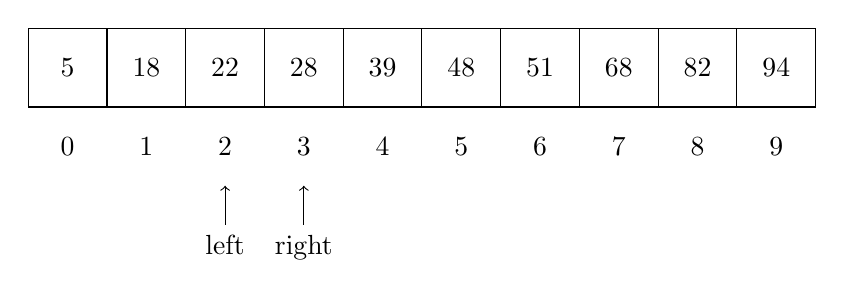
\begin{tikzpicture}
      \draw (0, 0) rectangle (1, 1);
      \node at (0.5, 0.5) {5};
      
      \draw (1, 0) rectangle (2, 1);
      \node at (1.5, 0.5) {18};
      
      \draw (2, 0) rectangle (3, 1);
      \node at (2.5, 0.5) {22};
      
      \draw (3, 0) rectangle (4, 1);
      \node at (3.5, 0.5) {28};
      
      \draw (4, 0) rectangle (5, 1);
      \node at (4.5, 0.5) {39};
      
      \draw (5, 0) rectangle (6, 1);
      \node at (5.5, 0.5) {48};
      
      \draw (6, 0) rectangle (7, 1);
      \node at (6.5, 0.5) {51};
      
      \draw (7, 0) rectangle (8, 1);
      \node at (7.5, 0.5) {68};
      
      \draw (8, 0) rectangle (9, 1);
      \node at (8.5, 0.5) {82};
      
      \draw (9, 0) rectangle (10, 1);
      \node at (9.5, 0.5) {94};

      \foreach \i in {0,1,...,9} {
        \node at (\i+0.5, -0.5) {\i};
    }

      % ラベルをはる
      \draw[<-] (2.5, -1) -- (2.5, -1.5) node[below] {left};
      \draw[<-] (3.5, -1) -- (3.5, -1.5) node[below] {right};
  \end{tikzpicture}
\end{center}

二分探索の実装は以下の通りです。

\begin{lstlisting}[caption=二分探索の実装, frame=TRBL, label={simle_binary}]
def binary_search(A: list[int], value: int) -> int:
    left, right = 0, len(A) - 1
    
    while left <= right:
        mid = (left + right) // 2
        
        if A[mid] == value:
            return mid
        
        if A[mid] < value:
            left = mid + 1
        else:
            right = mid - 1
    
    return -1
\end{lstlisting}

\subsection{一般化した二分探索}
Pythonの標準ライブラリであるbisectのbisect\_leftの実装をしましょう。bisect\_leftはソートされた配列に対して、
与えられた値以上の最小のindexを返す関数です。bisect\_leftは二分探索を用いて実装されています。先ほどの配列から要素を探す二分探索では、要素一致するか否かを判定していましたが、
今回はもっと一般化して「midがある条件を満たすか否か」を判定して範囲を狭めていきます。このとき、leftより右側の区間は
条件を満たさず、rightより左側の区間は条件を満たすようにします。 

二分探索では以下の図のような条件を満たす赤い部分を条件を満たす境界ギリギリになるように更新していきます。

\begin{itemize}
  \item leftは常に条件を満たさない
  \item rightは常に条件を満たす
\end{itemize}

という条件を満たすように処理を進めていき、最終的にleftが条件を満たさない最大のindex、rightが条件を満たす最小のindexを返します。
bisect\_leftではleftが与えられた値よりも小さく、rightが与えられた値以上の最小のindexを返す関数です。

\vspace{0.5cm}

\begin{center}
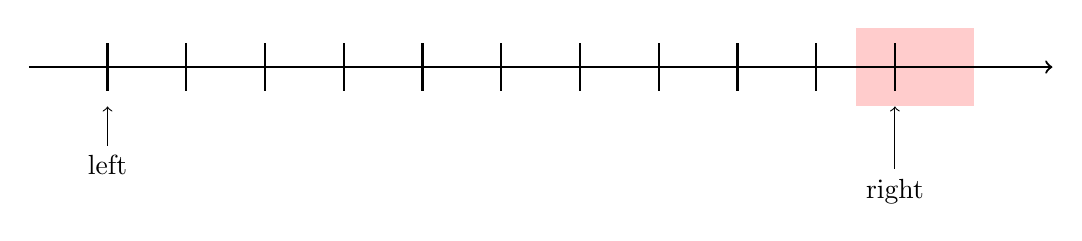
\begin{tikzpicture}
    \fill[red!20] (10.5, 0.5) rectangle (12, 1.5);
    \foreach \x in {1, 2, 3, 4, 5, 6, 7, 8, 9, 10, 11} {
        \draw[thick] (\x, 0.7) -- (\x, 1.3);
    }

    \draw[->, thick] (0, 1) -- (13, 1);
    \draw[<-] (1, 0.5) -- (1, -0.) node[below] {left};
    \draw[<-] (11, 0.5) -- (11, -0.3) node[below] {right};
\end{tikzpicture}
\end{center}

\begin{center}
  \textbf{初期状態}
\end{center}

\vspace{0.5cm}

\begin{center}
  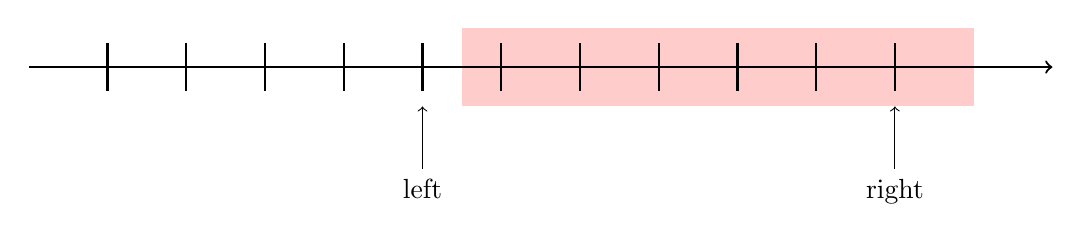
\begin{tikzpicture}
      \fill[red!20] (5.5, 0.5) rectangle (12, 1.5);
      \foreach \x in {1, 2, 3, 4, 5, 6, 7, 8, 9, 10, 11} {
          \draw[thick] (\x, 0.7) -- (\x, 1.3);
      }
  
      \draw[->, thick] (0, 1) -- (13, 1);
      \draw[<-] (5, 0.5) -- (5, -0.3) node[below] {left};
      \draw[<-] (11, 0.5) -- (11, -0.3) node[below] {right};
  \end{tikzpicture}
  \end{center}
  
  \begin{center}
    \textbf{終了状態}
  \end{center}

bisect\_leftの実装は以下の通りです。

\begin{lstlisting}[caption=bisect\_leftの実装, frame=TRBL, label={bisect_left}]
def bisect_left(array: list[int], key: int) -> int:
  left, right = -1, len(array)
  
  while right - left > 1:
      mid = (left + right) // 2
      
      if array[mid] < key:
          left = mid
      else:
          right = mid
  
  return right
\end{lstlisting}

bisect\_leftの実装では、左側が条件を満たさない、右側が条件を満たすといった実装になっています。これだとまだ条件次第でleftが条件を満たす、rightが条件を満たさないという
実装もあり得ます。そこで以下ではめぐる式二分探索のさらに一般化した実装を紹介します。

\subsection{めぐる式二分探索}

めぐる式二分探索では、

\begin{itemize}
  \item ngは常に条件を満たさない
  \item okは常に条件を満たす
\end{itemize}

のように数直線上の右や左という概念を持たせずに実装します。めぐる式二分探索は以下のように実装されます。
is\_okは条件を満たすかどうかを判定する関数ですので、条件に合わせて実装します。

\begin{lstlisting}[caption=めぐる式二分探索, frame=TRBL, label={megru}]
def binary_search(array: list[int], key: int):
    ng, ok = -1, len(array)
    
    while abs(ok - ng) > 1:
        mid = (ng + ok) // 2
        
        if is_ok(array, mid, key):
            ok = mid
        else:
            ng = mid
    
    return ok
\end{lstlisting}

\newpage

\section{二分探索木}
二分探索は探索自体は$O(\log n)$で行うことができますが、配列がソートされているひつようがあり、データの挿入や削除がある場合は毎回ソートがあり非効率ではあります。
解決策としては、\textbf{データ構造で解決}や\textbf{Treeq}などがあります。データ構造で解決する方法の一つが\textbf{二分探索木}です。

\textbf{二分探索木}は以下の性質を持った木構造です。

\begin{itemize}
  \item 左子ノードは親ノードよりも小さい(または等しい) (下の図では$B \leq A$)
  \item 右子ノードは親ノードよりも大きい (下の図では$A < C$)
\end{itemize}

\begin{center}
    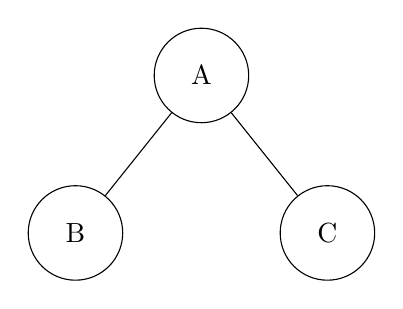
\begin{tikzpicture}[scale=0.4]
      \node[circle, draw, minimum size=1.2cm] (A) at (0, 0) {};
      \node[circle, draw, minimum size=1.2cm] (B) at (-4, -5) {};
      \node[circle, draw, minimum size=1.2cm] (C) at (4, -5) {};

      % 線を引く
      \draw (A) --(B);
      \draw (A) -- (C);

      % 値を入れる
      \node at (0, 0) {A};
      \node at (-4, -5) {B};
      \node at (4, -5) {C};
    \end{tikzpicture}
\end{center}

二分探索木で行う処理は以下の通りです。

\begin{itemize}
  \item 木の作成
  \item 探索
  \item 削除
\end{itemize}

\subsection{二分探索木の作成}
\texttt{[22,18, 5, 82, 51, 39]}の配列を二分探索木に変換してみましょう。

\vspace{0.5cm}

\begin{center}
  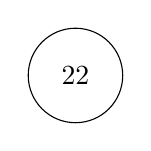
\begin{tikzpicture}
    \node[circle, draw, minimum size=1.2cm] (A) at (0, 0) {}; 

    % 値を入れる
    \node at (0, 0) {22};
  \end{tikzpicture}
\end{center}

\begin{center}
  \textbf{22を挿入}
\end{center}

\vspace{0.5cm}

\begin{center}
  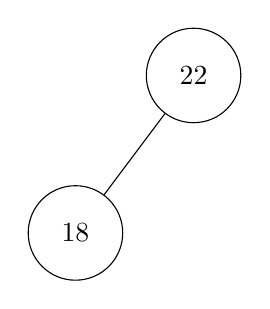
\begin{tikzpicture}
    \node[circle, draw, minimum size=1.2cm] (A) at (0, 0) {}; 
    \node[circle, draw, minimum size=1.2cm] (B) at (-1.5, -2) {};

    % 線を引く
    \draw (A) --(B);

    % 値を入れる
    \node at (0, 0) {22};
    \node at (-1.5, -2) {18};
  \end{tikzpicture}
\end{center}

\begin{center}
  \textbf{18を挿入}
\end{center}

\vspace{0.5cm}

\begin{center}
  \begin{tikzpicture}
    \node[circle, draw, minimum size=1.2cm] (A) at (0, 0) {}; 
    \node[circle, draw, minimum size=1.2cm] (B) at (-1.5, -2) {};
    \node[circle, draw, minimum size=1.2cm] (C) at (-3, -4) {};

    % 線を引く
    \draw (A) --(B);
    \draw (B) -- (C);

    % 値を入れる
    \node at (0, 0) {22};
    \node at (-1.5, -2) {18};
    \node at (-3, -4) {5};
  \end{tikzpicture}
\end{center}

\begin{center}
  \textbf{5を挿入}
\end{center}

\vspace{0.5cm}

\begin{center}
  \begin{tikzpicture}
    \node[circle, draw, minimum size=1.2cm] (A) at (0, 0) {}; 
    \node[circle, draw, minimum size=1.2cm] (B) at (-1.5, -2) {};
    \node[circle, draw, minimum size=1.2cm] (C) at (-3, -4) {};
    \node[circle, draw, minimum size=1.2cm] (D) at (1.5, -2) {};

    % 線を引く
    \draw (A) --(B);
    \draw (B) -- (C);
    \draw (A) -- (D);

    % 値を入れる
    \node at (0, 0) {22};
    \node at (-1.5, -2) {18};
    \node at (-3, -4) {5};
    \node at (1.5, -2) {82};
  \end{tikzpicture}
\end{center}

\begin{center}
  \textbf{82を挿入}
\end{center}

\vspace{0.5cm}

\begin{center}
  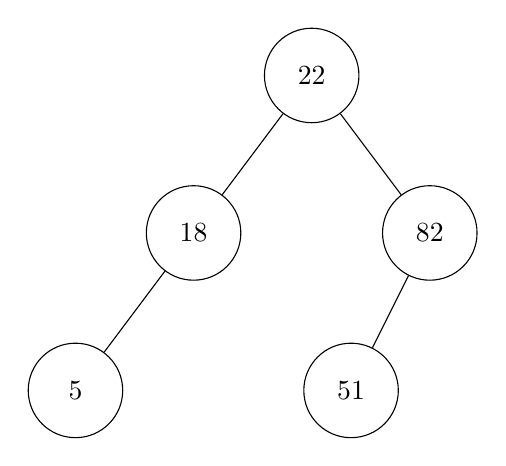
\begin{tikzpicture}
    \node[circle, draw, minimum size=1.2cm] (A) at (0, 0) {}; 
    \node[circle, draw, minimum size=1.2cm] (B) at (-1.5, -2) {};
    \node[circle, draw, minimum size=1.2cm] (C) at (-3, -4) {};
    \node[circle, draw, minimum size=1.2cm] (D) at (1.5, -2) {};
    \node[circle, draw, minimum size=1.2cm] (E) at (0.5, -4) {};

    % 線を引く
    \draw (A) --(B);
    \draw (B) -- (C);
    \draw (A) -- (D);
    \draw (D) -- (E);

    % 値を入れる
    \node at (0, 0) {22};
    \node at (-1.5, -2) {18};
    \node at (-3, -4) {5};
    \node at (1.5, -2) {82};
    \node at (0.5, -4) {51};
  \end{tikzpicture}
\end{center}

\begin{center}
  \textbf{51を挿入}
\end{center}

\vspace{0.5cm}

\begin{center}
  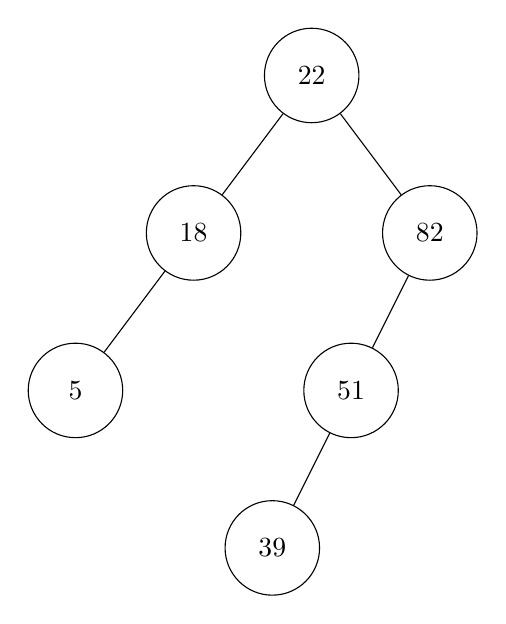
\begin{tikzpicture}
    \node[circle, draw, minimum size=1.2cm] (A) at (0, 0) {}; 
    \node[circle, draw, minimum size=1.2cm] (B) at (-1.5, -2) {};
    \node[circle, draw, minimum size=1.2cm] (C) at (-3, -4) {};
    \node[circle, draw, minimum size=1.2cm] (D) at (1.5, -2) {};
    \node[circle, draw, minimum size=1.2cm] (E) at (0.5, -4) {};
    \node[circle, draw, minimum size=1.2cm] (F) at (-0.5, -6) {};

    % 線を引く
    \draw (A) --(B);
    \draw (B) -- (C);
    \draw (A) -- (D);
    \draw (D) -- (E);
    \draw (E) -- (F);

    % 値を入れる
    \node at (0, 0) {22};
    \node at (-1.5, -2) {18};
    \node at (-3, -4) {5};
    \node at (1.5, -2) {82};
    \node at (0.5, -4) {51}; 
    \node at (-0.5, -6) {39};

  \end{tikzpicture}
\end{center}

\begin{center}
  \textbf{39を挿入}
\end{center}

\subsection{二分探索木の探索}
上の木を例に51を探してみましょう。根から順に探していきます。
\vspace{0.5cm}

\begin{center}
  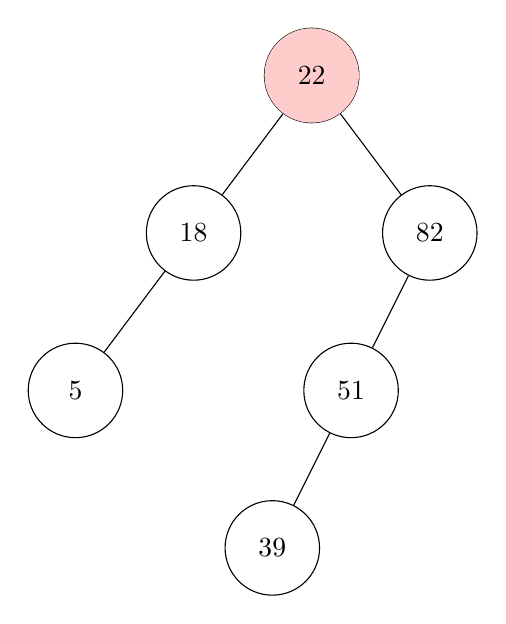
\begin{tikzpicture}
    \node[circle, draw, minimum size=1.2cm] (A) at (0, 0) {}; 
    \node[circle, draw, minimum size=1.2cm] (B) at (-1.5, -2) {};
    \node[circle, draw, minimum size=1.2cm] (C) at (-3, -4) {};
    \node[circle, draw, minimum size=1.2cm] (D) at (1.5, -2) {};
    \node[circle, draw, minimum size=1.2cm] (E) at (0.5, -4) {};
    \node[circle, draw, minimum size=1.2cm] (F) at (-0.5, -6) {};

    % 色を塗る
    \fill[red!20] (0, 0) circle (0.6);

    % 線を引く
    \draw (A) --(B);
    \draw (B) -- (C);
    \draw (A) -- (D);
    \draw (D) -- (E);
    \draw (E) -- (F);

    % 値を入れる
    \node at (0, 0) {22};
    \node at (-1.5, -2) {18};
    \node at (-3, -4) {5};
    \node at (1.5, -2) {82};
    \node at (0.5, -4) {51}; 
    \node at (-0.5, -6) {39};

  \end{tikzpicture}
\end{center}

\vspace{0.5cm}

51は22よりも大きいので右の子ノードに進みます。

\begin{center}
  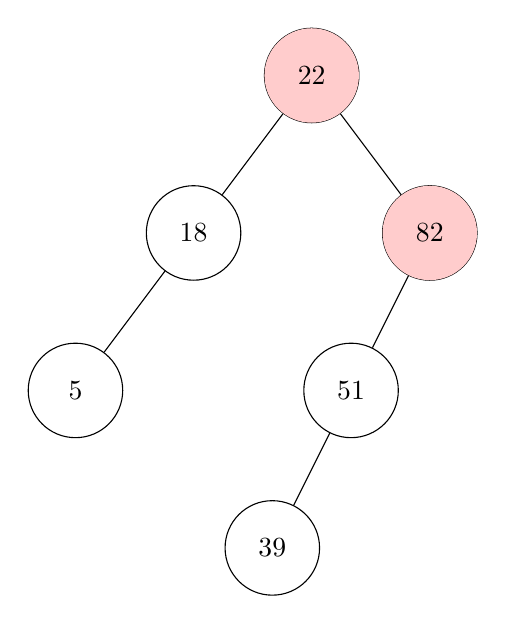
\begin{tikzpicture}
    \node[circle, draw, minimum size=1.2cm] (A) at (0, 0) {}; 
    \node[circle, draw, minimum size=1.2cm] (B) at (-1.5, -2) {};
    \node[circle, draw, minimum size=1.2cm] (C) at (-3, -4) {};
    \node[circle, draw, minimum size=1.2cm] (D) at (1.5, -2) {};
    \node[circle, draw, minimum size=1.2cm] (E) at (0.5, -4) {};
    \node[circle, draw, minimum size=1.2cm] (F) at (-0.5, -6) {};

    % 色を塗る
    \fill[red!20] (0, 0) circle (0.6);
    \fill[red!20] (1.5, -2) circle (0.6);

    % 線を引く
    \draw (A) --(B);
    \draw (B) -- (C);
    \draw (A) -- (D);
    \draw (D) -- (E);
    \draw (E) -- (F);

    % 値を入れる
    \node at (0, 0) {22};
    \node at (-1.5, -2) {18};
    \node at (-3, -4) {5};
    \node at (1.5, -2) {82};
    \node at (0.5, -4) {51}; 
    \node at (-0.5, -6) {39};

  \end{tikzpicture}
\end{center}

51は82よりも小さいので左の子ノードに進みます。見つかりました。

\vspace{0.5cm}

\begin{center}
  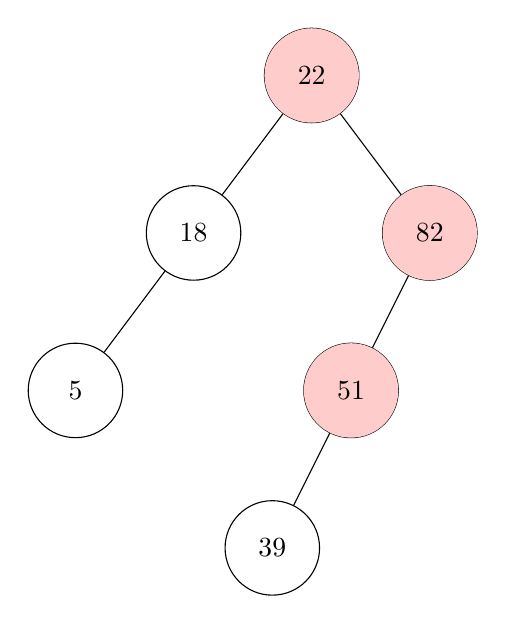
\begin{tikzpicture}
    \node[circle, draw, minimum size=1.2cm] (A) at (0, 0) {}; 
    \node[circle, draw, minimum size=1.2cm] (B) at (-1.5, -2) {};
    \node[circle, draw, minimum size=1.2cm] (C) at (-3, -4) {};
    \node[circle, draw, minimum size=1.2cm] (D) at (1.5, -2) {};
    \node[circle, draw, minimum size=1.2cm] (E) at (0.5, -4) {};
    \node[circle, draw, minimum size=1.2cm] (F) at (-0.5, -6) {};

    % 色を塗る
    \fill[red!20] (0, 0) circle (0.6);
    \fill[red!20] (1.5, -2) circle (0.6);
    \fill[red!20] (0.5, -4) circle (0.6);

    % 線を引く
    \draw (A) --(B);
    \draw (B) -- (C);
    \draw (A) -- (D);
    \draw (D) -- (E);
    \draw (E) -- (F);

    % 値を入れる
    \node at (0, 0) {22};
    \node at (-1.5, -2) {18};
    \node at (-3, -4) {5};
    \node at (1.5, -2) {82};
    \node at (0.5, -4) {51}; 
    \node at (-0.5, -6) {39};

  \end{tikzpicture}
\end{center}

\subsection{二分探索木の削除}

二分探索木からノードを削除する場合は以下の3つのケースがあります。

\begin{itemize}
  \item 子ノードがない場合
  \item 子ノードが1つの場合
  \item 子ノードが2つの場合
\end{itemize}

\subsubsection{子ノードがない場合}
例えば5を削除する場合を考えます。5は左右の子ノードがないので、他のノードに影響がないためそのまま削除します。

\begin{center}
  \begin{tikzpicture}
    \node[circle, draw, minimum size=1.2cm] (A) at (0, 0) {}; 
    \node[circle, draw, minimum size=1.2cm] (B) at (-1.5, -2) {};
    \node[circle, draw, minimum size=1.2cm, dotted] (C) at (-3, -4) {};
    \node[circle, draw, minimum size=1.2cm] (D) at (1.5, -2) {};
    \node[circle, draw, minimum size=1.2cm] (E) at (0.5, -4) {};
    \node[circle, draw, minimum size=1.2cm] (F) at (-0.5, -6) {};

    % 線を引く
    \draw (A) --(B);
    \draw [dotted] (B) -- (C);
    \draw (A) -- (D);
    \draw (D) -- (E);
    \draw (E) -- (F);

    % 値を入れる
    \node at (0, 0) {22};
    \node at (-1.5, -2) {18};
    \node at (-3, -4) {5};
    \node at (1.5, -2) {82};
    \node at (0.5, -4) {51}; 
    \node at (-0.5, -6) {39};

  \end{tikzpicture}
\end{center}

\subsubsection{子ノードが1つの場合}
次に18を削除する場合を考えます。18は左の子ノードが5しか持っていないので、5を18の位置に移動させます。18は親ノードから見て
左の子ノードですが、右ノードの場合も同様に処理します。

\vspace{0.5cm}

\begin{center}
  \begin{tikzpicture}
    \node[circle, draw, minimum size=1.2cm] (A) at (0, 0) {}; 
    \node[circle, draw, minimum size=1.2cm] (B) at (-1.5, -2) {};
    \node[circle, draw, minimum size=1.2cm, dotted] (C) at (-3, -4) {};
    \node[circle, draw, minimum size=1.2cm] (D) at (1.5, -2) {};
    \node[circle, draw, minimum size=1.2cm] (E) at (0.5, -4) {};
    \node[circle, draw, minimum size=1.2cm] (F) at (-0.5, -6) {};

    % 線を引く
    \draw (A) --(B);
    \draw [dotted] (B) -- (C);
    \draw (A) -- (D);
    \draw (D) -- (E);
    \draw (E) -- (F);

    % 値を入れる
    \node at (0, 0) {22};
    \node at (-1.5, -2) {5};
    \node at (-3, -4) {};
    \node at (1.5, -2) {82};
    \node at (0.5, -4) {51}; 
    \node at (-0.5, -6) {39};

  \end{tikzpicture}
\end{center}

\subsubsection{子ノードが2つの場合}
最後に22を削除する場合を考えます。削除するノードが2つの子ノードを持っている場合は、削除するノードの左の子ノードの最大値か、右の子ノードの最小値を持ってきて、
削除するノードに移動させます。ここでは、22の右の子ノードの最小値39を持ってきて、22の位置に移動させます。

\vspace{0.5cm}

\begin{center}
  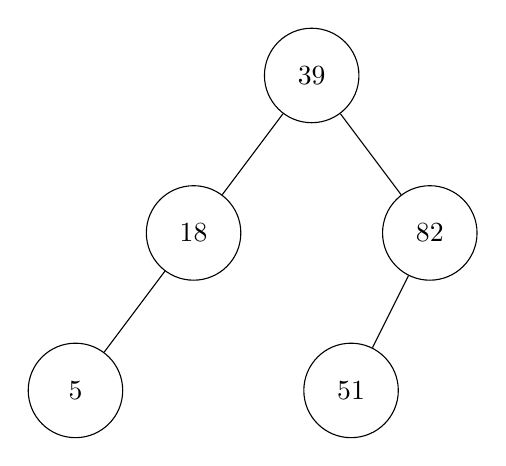
\begin{tikzpicture}
    \node[circle, draw, minimum size=1.2cm] (A) at (0, 0) {}; 
    \node[circle, draw, minimum size=1.2cm] (B) at (-1.5, -2) {};
    \node[circle, draw, minimum size=1.2cm] (C) at (-3, -4) {};
    \node[circle, draw, minimum size=1.2cm] (D) at (1.5, -2) {};
    \node[circle, draw, minimum size=1.2cm] (E) at (0.5, -4) {};

    % 線を引く
    \draw (A) --(B);
    \draw (B) -- (C);
    \draw (A) -- (D);
    \draw (D) -- (E);

    % 値を入れる
    \node at (0, 0) {39};
    \node at (-1.5, -2) {18};
    \node at (-3, -4) {5};
    \node at (1.5, -2) {82};
    \node at (0.5, -4) {51}; 

  \end{tikzpicture}
\end{center}

\subsection{二分木の実装}
\begin{lstlisting}[caption=二分木の実装, frame=TRBL, label={binary_tree}]
class Node:
  def __init__(self, data: int) -> None:
      self.data: int = data
      self.right: Node | None = None
      self.left: Node | None = None
      
  def __str__(self) -> str:
      return str(self.data)
  
class BinarySearchTree:
  def __init__(self):
      self.root = None
      
  def create(self, array: list[int]) -> None:
      for i in range(len(array)):
          self.insert(array[i])
  
  def insert(self, data: int) -> None:
      if self.root is None:
          self.root = Node(data)
      else:
          self._insert_recursively(self.root, data)
  
  def _insert_recursively(self, node: Node, data: int) -> None:
      if data <= node.data:
          if node.left is None:
              node.left = Node(data)
          else:
              self._insert_recursively(node.left, data)
      else:
          if node.right is None:
              node.right = Node(data)
          else:
              self._insert_recursively(node.right, data)
  
  def search(self, value: int) -> Node | None:
      if self.root is None:
          return self.root
      
      return self._search_recursively(self.root, value)
      
  def _search_recursively(self, node: Node, value: int) -> Node | None:
      if node.data == value:
          return node
      
      if value < node.data:
          if node.left is None:
              return node.left
          else:
              return self._search_recursively(node.left, value)
      else:
          if node.right is None:
              return node.right
          else:
              return self._search_recursively(node.right, value)
  
  def delete(self, value: int) -> Node | None:
      if self.root is None:
          return self.root
      else:
          self.root = self._delete_recursively(self.root, value)
  
  def _delete_recursively(self, node: Node, value: int) -> Node | None:
      if value < node.data:
          if node.left is None:
              return None
          else:
              node.left = self._delete_recursively(node.left, value)
      elif value > node.data:
          if node.right is None:
              return None
          else:
              node.right = self._delete_recursively(node.right, value)
      else:
          if node.left is None and node.right is None:
              return None
          elif node.left is None:
              return node.right
          elif node.right is None:
              return node.left
          else:
              successor = self._successor()
              node.data = successor.data
              self._delete_recursively(node.right, successor.data)
              
      return node
  
  def _successor(self) -> Node | None:
      if self.root is None:
          return self.root
      
      node = self.root
      
      while node.left is not None:
          node = node.left
      
      return node
\end{lstlisting}

\newpage

\section{平衡木}

\section{参考}
\textbf{二分探索}

\begin{itemize}
  \item \url{https://qiita.com/drken/items/97e37dd6143e33a64c8c}
\end{itemize}


\end{document}